% TEMPLATE for Usenix papers, specifically to meet requirements of
%  USENIX '05
% originally a template for producing IEEE-format articles using LaTeX.
%   written by Matthew Ward, CS Department, Worcester Polytechnic Institute.
% adapted by David Beazley for his excellent SWIG paper in Proceedings,
%   Tcl 96
% turned into a smartass generic template by De Clarke, with thanks to
%   both the above pioneers
% use at your own risk.  Complaints to /dev/null.
% make it two column with no page numbering, default is 10 point

% Munged by Fred Douglis <douglis@research.att.com> 10/97 to separate
% the .sty file from the LaTeX source template, so that people can
% more easily include the .sty file into an existing document.  Also
% changed to more closely follow the style guidelines as represented
% by the Word sample file. 

% Note that since 2010, USENIX does not require endnotes. If you want
% foot of page notes, don't include the endnotes package in the 
% usepackage command, below.

% This version uses the latex2e styles, not the very ancient 2.09 stuff.
\documentclass[letterpaper,10pt]{article}
\usepackage{epsfig,graphicx,usenix,fullpage,float,hyperref}
\usepackage{mathtools,amssymb,setspace, pbox}
\usepackage[table,xcdraw]{xcolor}
\usepackage[center, labelfont=bf]{caption}

\DeclarePairedDelimiter{\ceil}{\lceil}{\rceil}
\DeclarePairedDelimiter{\floor}{\lfloor}{\rfloor}
\def\bE{\mathbb{E}}

%\usepackage{endnotes}
\begin{document}


%make title bold and 14 pt font (Latex default is non-bold, 16 pt)
\title{\Large \bf 6.824 Final Project}
%for single author (just remove % characters)
\author{
{\rm Colleen Josephson}\\
cjoseph@mit.edu
\and
{\rm Joseph DelPreto}\\
delpreto@mit.edu
\and
{\rm Pranjal Vachaspati}\\
pranjal@mit.edu
\and
{\rm Steven Valdez}\\
dvorak42@mit.edu
% copy the following lines to add more authors
% \and
% {\rm Name}\\
%Name Institution
} % end author

\date{May 11, 2014}

\maketitle

% Use the following at camera-ready time to suppress page numbers.
% Comment it out when you first submit the paper for review.
%\thispagestyle{empty}

\section{Introduction}
The presented project implements a persistent, fault-tolerant,
high-performance key/value store. In order to achieve these goals, the
system implements at-most-once semantics, relies upon Paxos for
reaching consenus, shards the database across multiple replica groups,
persistently stores values to disk, and implements protocols for
automatically recovering and updating disk contents upon server
reboot.  In order to improve performance, the system features two
paxos optimizations: a protocol similar to multi-paxos to avoid the
dueling leaders problem, and the ability for leaders to send out
prepare messages in advance to reduce the required number of RPCs for
paxos agreeement.

Extensive testing was done to evaluate the system's persistence,
recovery, and performance by extending existing tests and creating new
ones.  After modifying the local RPC system to work on a real network,
the system was deployed on an Amazon Web Services (AWS) cluster to
obtain realistic measurements of throughput, latency, and disk
recovery speed.

Source code for this project is accessible at \url{https://github.com/pranjalv123/mexos}.

\section{Design} \label{sec:design} The design is based upon the code
developed throughout the semester for lab 4.  There are therefore
three basic components running on each server: Paxos processes to
reach consenus for instances, a shard master to determine which groups
are responsible for various shards of the database, and a shard
key/value storage process to execute client Put/Get requests.  The
Paxos instances are used to create a consistent log of operations for
both shard reconfiguration and client operations.

Battery tests were run to determine which combination of our prior
labs created the fastest and most reliable starting point.  Once a
working codebase was compiled, modifications were made to address
three major areas: Paxos optimizations, persistence (with disk
recovery), and testing over a real network on AWS.

\subsection{Paxos Optimizations}
In order to improve the performance of Paxos, we implemented the
Multi-Paxos leader selection optimization. This optimization solved
the dueling leaders problem, preventing us from hanging forever in a
loop between conflicting leaders, and also allowed us to reduce the
number of RPC calls that were necessary to come to agreement, by
allowing us to skip the Prepare phase of the Paxos protocol for a
leader that was constant between instances. The main issue with the
Multi-Paxos leader selection is ensuring that leadership information
is propogated through the system and ensuring that we never agree as
part of two separate partitions when the Prepare phase is
skipped. Unfortunately, we discovered a number of implementation bugs
with our default Paxos implementation, which we ended up fixing to end
up with a fairly reliable Multi-Paxos optimized system that had a
selected leader and skipped unnecessary prepare phases. The results
were that the number of required RPCs was reduced by about 33\%, and
that there were reduced bandwidth requirements due to the singular
leadership. There was an issue that a single machine became the
primary proposer, potentially limiting it based on disk and processor
speeds, however this doesn't appear to be an issue at the anticipated
use cases.

\subsection{Persistent Storage}
In order to tolerate servers restarting and to handle databases that
cannot fit in memory, all three components of the system store state
and data persistently on disk.  To interface with the disk, a Go
wrapper for the high-performance C++ key/value libray LevelDB was
utilized.  An outline of what each system component stores on disk is
presented below.
\begin{itemize}
\item The Paxos processes write the highest accepted value, the
  highest accepted proposal number, and the highest acknowledged
  prepare request to disk for each instance.  This ensures that the
  protocol will operate correctly even if a server restarts \cite{paxos} (for
  example, a decided value can never be changed).  In addition to this
  state, the Paxos processes persistently store the done responses
  received from peers and the number of the maximum known instance
  (see the recovery section below).

\item The shard master writes every configuration to disk, ensuring
  that will be able to respond to historical queries even after
  restarting.  In addition, it stores the highest executed Paxos log
  entry and the number of its highest known configuration.

\item The shard key/value service writes its database to disk by
  writing each value as each Put request is executed.  In addition, it
  must preserve at-most-once semantics and consistency across reboots,
  so it persistently stores which operations have been seen as well as
  the most recent response sent to each client.  It also writes the
  highest executed Paxos log entry and the current configuration
  number.
\end{itemize}

In all cases, the specified data is written to disk before returning
to the caller, so any response that a caller receives from a peer will
not be forgotten by the responder even if it restarts.  It may be the
case that the responder crashes before sending the response, but this
is acceptable since the system offers at-most-once semantics (so the
caller must be prepared to retry and the responder is prepared to
filter duplicates).

\subsubsection{Recovery from Failures}
In order to tolerate servers restarting with or without their disk
contents, the system includes protocols for recovering and catching up
on startup.  These can be summarized by considering what happens when
a server starts:

\begin{itemize}
\item The Paxos process will load any saved done responses and maximum
  instance number from its disk.  It will then contact peers to
  request their done responses and maximum instance number,
  determining which peer is the most updated out of any peers that
  respond.  From these values, both the ones read from disk and the
  ones received, it can determine which instances it should know about
  but does not; it then requests these instances from its peers.
\item The shard master process will load the highest known
  configuration and highest executed Paxos log instance from disk if
  it exists.  It will then request the same information from its
  peers, determining who among the responders is the most updated.
  From this information it can determine if there are any missed
  configurations, and if so request them from a peer.
\item The shard key/value service will load its last known
  configuration and the highest executed Paxos log instance from disk
  if it exists.  It will then request the same information from peers,
  determining the most updated state that it should have.  Finally, it
  can request the actual database key/value entries from a peer (see
  below for details of how this transfer is performed) along with any
  client responses and lists of seen operations.
\end{itemize}

These protocols allow any number of servers restarting with their disk contents to catch themselves up from any updated peer.  They also allow any number of servers restarting without their disk contents to recover the needed data from any peer that has the data.

\textbf{Single server crashing and restarting, disk intact or lost}: As described above, each
recovery process contacts a random replica in the same replica group.  The recovering server can then get any missing data by comparing states with the updated server (e.g. shard data, shard master configurations, and Paxos instances - note that Paxos only discards old decisions if all participants have marked that sequence number as 'done').  This will therefore work regardless of whether the disk was lost or simply out of date.  Note that when data is transferred, multiple messages may be used for a single shard if it is too large to fit in memory - the sender will periodically check memory usage while constructing the reply and mark replies as incomplete if needed.

% Is the below actually implemented?
%The recovery process contacts a random replica in the same replica group, and tells the up-to-date server that it has no state. The two servers open an auxiliary TCP connection to send over the relevant portions of the database. This avoids RPC overhead, since the database might be large. The database has an in-order iterator, in case the TCP connection fails, the recoverer can re-establish the connection and ask the sender to pick up where it left off. If the sending server fails, then the recovering server asks a new replica. This allows for a failure mode where the original server remains locked permanently. We have decided that this is preferable to sacrificing consistency, and the system administrator can resolve the problem by rebooting the hung server.

\textbf{Complete crash of all servers}: If all servers lose their disk state, then all will restart and begin like a brand new deployment (the above protocols will simply not find any updated data to transfer). If the disks are not lost, then the recovery process will read the various states written to disk and pick up where it left off.  Because disk writes take place before any operation commits, data is not lost.

It should be noted that during a shard transfer (including recovery), the shard key/value service on both the sender and recoverer ignore client requests in order to ensure that consistent data is sent (their databases cannot be modified except through the recovery process itself).  Since their Paxos processes continue running independently, however, progress can still be made even if a majority of servers is involved in a data transfer (the decided operations will be persistently logged and the halted servers can catch up when transfer is complete).  This therefore improves performance during recoveries or transfers.

In addition, effort was made to utilize memory in addition to the
disk in order to increase performance.  The LevelDB database has
the option to use a least-recently-used (LRU) cache to store
recently used entries in memory.  In addition, a configuration
variable was added to the service to allow values to be written to
memory as well as disk until the memory is full.  These two
options, combined with the native cache of the operating system,
allow many needed values to be read quickly from memory rather than
always consulting the disk.

\subsection{Testing}
About 25 new tests were created, and existing ones were extended, in order to evaluate persistent storage and run on TCP sockets instead of unix file sockets.  A few flags and configuration variables can select different modes (e.g. with and without persistence, RPC using unix file sockets or localhost TCP).

Below are summaries of different located at 'mexos/src/\emph{$<$name$>$}/test\_test.go' unless otherwise noted.

\emph{paxos:} Paxos specific tests which include restarting servers deterministically or randomly.  These include cases where servers lose their disks, where all servers restart, where partitioning changes, where communication is unreliable, and many combinations of the above.  There are also benchmarks for measuring performance.

\emph{shardmaster:} Shardmaster specific tests which include restarting servers with or without disk to ensure that persistence and recovery work as expected.  There are also benchmarks for measuring performance.

\emph{shardkv:} Shardkv specific tests which include deterministically restarting servers to ensure that persistence and recovery operate correctly.  There is also a test which performs the previously written tests but with random reboots of random servers or entire groups.  There are also benchmarks for measuring shard transfer speed and to ensure that the simulated memory limit is never exceeded.

\emph{test:} Tests and benchmarks modified to run on our AWS cluster.  Running these tests are the most complicated, and require the user to SSH into the AWS cluster leader and start the servers on other cluster machines using 'start-on-all.sh' to run 'mexos/src/main/start.go'. These tests required a surprising amount of debugging and glue code.  Additionally, to check for correct operation under server failure, backdoor RPCs were required to tell a remote server to act deaf or dead.

The results of these benchmarks are presented below.

\section{Performance}

An extensive testing system was created to try and accurately measure performance.  This comprises many new benchmarks, as well as a modified RPC system to run the servers in an AWS cluster and observe the performance on a real network.

\subsection{Server Configuration}
Two Amazon AWS clusters were provisioned to test real-life performance of the system. The faster of the clusters used Amazon's m3.large instance type, where each server has 7.5 gigabytes of RAM, 2 Intel Xeon i5 Sandy Bridge CPU cores, and 1 32 gigabyte solid state drive. Real-world network performance, measured using iperf, was approximately 700 Mb/s. The slower of the clusters used Amazon's m1.small instance type, where each server has 1.7 gigabytes of RAM, 1 Intel Xeon Westmere core, and 1 160 gigabyte hard disk drive. Real-world network performance was approximately 150 Mb/s. Each cluster had one control node and twelve slave nodes. Instances were allocated on multi-tenant hardware, and nodes within a cluster were within the same region and availability zone.

\subsection{Throughput and Latency}

Performance tests were run using both vanilla paxos and multipaxos under a variety of conditions. The tests were run on an actual network in an AWS cluster. 

\textit{Client latency}: Average time it takes for one client to see a
request processed. 

\textit{Throughput}: Number of requests, on average, the
client will see processed in a second.

\textit{System throughput}: Number of requests per second the entire system can handle. This is different than the client throughput because clients always wait to see the response of the current request before dispatching another.

System throughput requires a saturation of multiple clients sending continuous requests for a certain amount of time (here, ten seconds). The system saturated from 10 to 50 clients, depending on the number of groups/replicas. After the saturation point, adding more clients
causes a decrease in throughput because of network traffic saturation.

Some tests were repeatedly run on one key, and others on a random set of keys. This helps indicate how the performance changes when requests all go to the same replica group versus when they are evenly spread across all replica groups.

% Please add the following required packages to your document preamble:
% \usepackage[table,xcdraw]{xcolor}
% If you use beamer only pass ``xcolor=table'' option, i.e. \documentclass[xcolor=table]{beamer}
\begin{table}
\begin{tabular}{|l|l|l|l|}
\hline
\multicolumn{4}{|c|}{\cellcolor[HTML]{C0C0C0}{\color[HTML]{000000} \textbf{Vanilla Paxos}}}                           \\ \hline
                              & \textbf{Avg. Client Latency} & \textbf{Avg. Client Throughput} & \textbf{System Throughput} \\ \hline
\multicolumn{4}{|c|}{\textit{PutHash to one key}}                                                                     \\ \hline
\textbf{1 group, 3 replicas}  & 40.3 ms/op                   & 24.8 requests/s              & 27 requests/s           \\ \hline
\textbf{1 group, 10 replicas} & 5370 ms/op                   & 0.18 requests/s              & 2 requests/s            \\ \hline
\textbf{3 groups, 3 replicas} & 62 ms/op                     &                              & 22 requests/s           \\ \hline
\multicolumn{4}{|c|}{\textit{PutHash to many keys}}                                                                   \\ \hline
\textbf{1 group, 3 replicas}  & 40.7 ms/op                   & 24.5 requests/s              & 30 requests/s           \\ \hline
\textbf{1 group, 10 replicas} & 282 ms/op                    & 3.5 requests/s               & 7 requests/s            \\ \hline
\textbf{3 groups, 3 replicas} & 214 ms/op                    & 4.6 requests/s               & 67 requests/s           \\ \hline
\end{tabular}
\end{table}

% Please add the following required packages to your document preamble:
% \usepackage[table,xcdraw]{xcolor}
% If you use beamer only pass ``xcolor=table'' option, i.e. \documentclass[xcolor=table]{beamer}
\begin{table}
\begin{tabular}{|l|l|l|l|}
\hline
\multicolumn{4}{|c|}{\cellcolor[HTML]{C0C0C0}{\color[HTML]{000000} \textbf{Multipaxos}}}                              \\ \hline
                              & \textbf{Avg. Client Latency} & \textbf{Avg. Client Throughput} & \textbf{System Throughput} \\ \hline
\multicolumn{4}{|c|}{\textit{PutHash to one key}}                                                                     \\ \hline
\textbf{1 group, 3 replicas}  & 27 ms/op                     & 37 requests/s                & 47 requests/s           \\ \hline
\textbf{1 group, 10 replicas} & 2360 ms/op                   & 0.42 requests/s              & 3.4 requests/s          \\ \hline
\textbf{3 groups, 3 replicas} & 22 ms/op                     & 45 requests/s                & 45 requests/s           \\ \hline
\multicolumn{4}{|c|}{\textit{PutHash to many keys}}                                                                   \\ \hline
\textbf{1 group, 3 replicas}  & 25 ms/op                     & 40 requests/s                & 45 requests/s           \\ \hline
\textbf{1 group, 10 replicas} & 130 ms/op                    & 7 requests/s                 & 10.3 requests/s         \\ \hline
\textbf{3 groups, 3 replicas} & 40 ms/op                     & 25 requests/s                & 124 requests/s          \\ \hline
\end{tabular}
\end{table}

It can be seen that, in all cases, the Paxos optimizations had a significant positive impact on both latency and client and system throughput.  For example, system throughput increased by an average of over 71\%.

For a single group case, the difference between three replicas and ten is striking.  With more replicas, more traffic is needed for a paxos agreement and thus latency increases.  Figure 1 demonstrates how throughput suffers as the number of replicas increases.  Another interesting effect is that as the number of replicas increases, the gap between the single key and multi-key cases increases dramatically even when there is a single group (and therefore all puts touch the same servers).

\begin{figure}[h]
\centering
\makebox[\textwidth][c]{
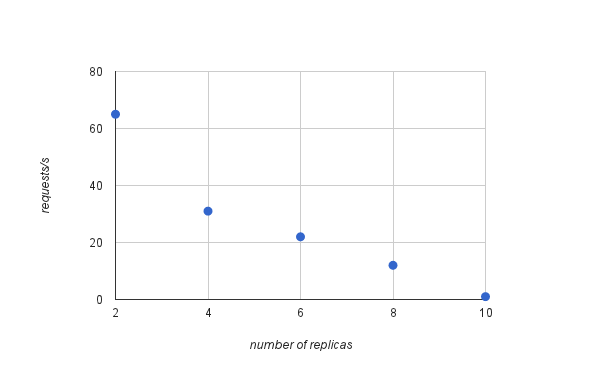
\includegraphics[scale=.40]{replicas.png}}
\caption{Performance of a one-group configuration rapidly deteriorates as the number of replicas increases}
\label{fig:replicas}
\end{figure}

Adding more groups, however, increases throughput.  For evenly distributed traffic, going from one group to 3 nearly triples the throughput when using multiple keys (thereby leveraging the additional groups).  Figure 2 shows that this trend continues, such that adding groups linearly improves the throughput of the system. The table shows that average throughput for a single client may suffer, probably because the system throughput benchmark creates many clients, while the client throughput test creates a single client; having multiple clients increases the likelihood that a client must wait to see its request served since the replicas may be busy serving another client's request.

\begin{figure}[h]
\centering
\makebox[\textwidth][c]{
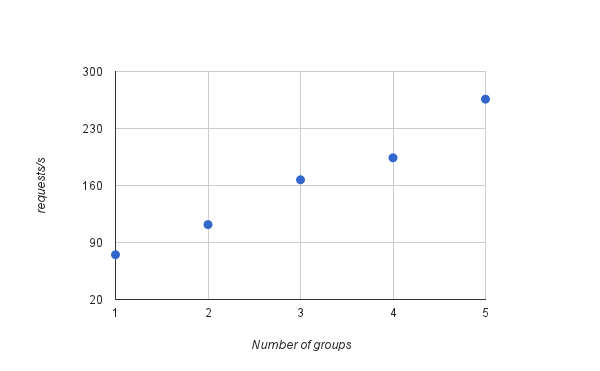
\includegraphics[scale=.4]{groups.png}}
\caption{Performance increases linearly as the number of groups increases. There is probably a saturation point, but we didn't have enough cluster machines to reach it.}
\label{fig:groups}
\end{figure}

\subsubsection{Paxos RPC Counts}

Utilizing optimizations similar to Multipaxos decreases the number of RPCs needed to reach agreement.

% Please add the following required packages to your document preamble:
% \usepackage[table,xcdraw]{xcolor}
% If you use beamer only pass ``xcolor=table'' option, i.e. \documentclass[xcolor=table]{beamer}
\begin{table}[h]
\centering
\makebox[\textwidth][c]{
\begin{tabular}{|l|l|l|}
\hline
\multicolumn{3}{|c|}{\cellcolor[HTML]{C0C0C0}\textbf{Paxos RPC Counts}}                  \\ \hline
                                 & \textbf{Single Proposer} & \textbf{Multiple Proposers} \\ \hline
\textbf{Normal Paxos}            & 30                       & 89            \\ \hline
\textbf{Paxos with Leaders}      & 20                       & 27                         \\ \hline
\textbf{Leaders and Pre-prepare} & 17                       & 20                         \\ \hline
\end{tabular}
}
\end{table}

\subsubsection{Disk Recovery}
Various tests were performed to evaluate the recovery time for servers restarting.  The AWS servers can either have hard disk drives or solid state drives, and both were evaluated for raw disk speed by writing 1GB of data to the database.  A HDD averaged about 47.7 MB/s while the SSD averaged about 166.6 MB/s.  The recovery was then tested by creating a one-group service, placing 100 MB worth of data in the database, and finally restarting a replica without its disk contents.  Various tests were run with differently sized values (and therefore differing numbers of entries).  In all tests, the memory limit was set to under 75 MB, so that data transfer was forced to take place using multiple messages.

\begin{table}
\begin{tabular}{|l|l|l|l|}
\hline
\multicolumn{4}{|c|}{\cellcolor[HTML]{C0C0C0}{\color[HTML]{000000} \textbf{Recovery Performance for 100MB Database}}}                           
\\ \hline \textbf{Value Size (KB)} &  \textbf{Number of Entries} & \textbf{Time Reading Database (s)} & \textbf{Recovery Time (s)} 
\\ \hline 5  & 20352 & 464.7 & ?
\\ \hline 50  & 2046 & 30.8 & 37.2
\\ \hline 100  & 1023 & 15.9 & 21.1
\\ \hline 150  & 682 & 10.2 & 15.8
\\ \hline 250  & 409 & 6.3 & 12.4
\\ \hline 500  & 204 & 3.5 & 10.6
\\ \hline 1024  & 99 & 1.88 & 8.3
\\ \hline 1500  & 68 & 1.4 & ?
\\ \hline
\end{tabular}
\end{table}

\begin{figure}[h]
\centering
\makebox[\textwidth][c]{
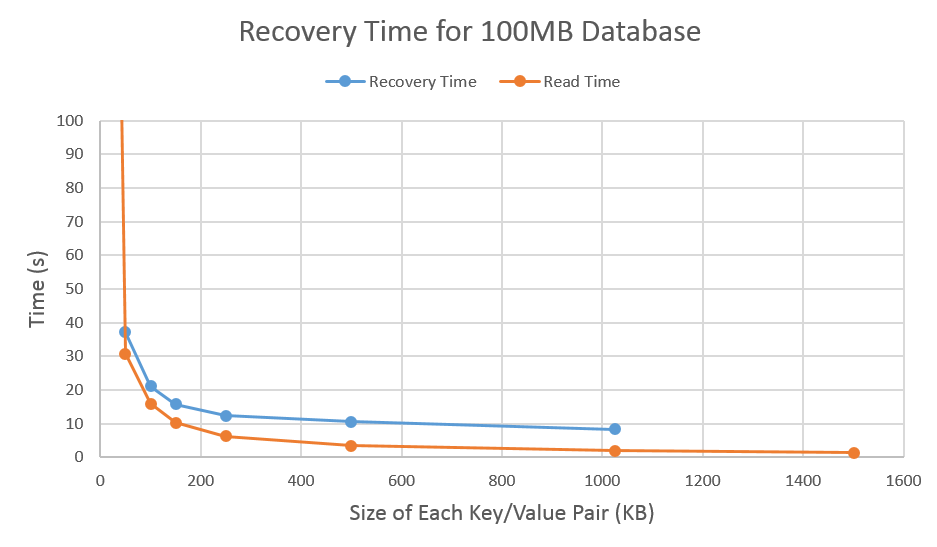
\includegraphics[scale=.7]{recovery.png}}
\caption{Performance increases dramatically as the number of keys is reduced (and the size of entries is increased).}
\label{fig:recovery}
\end{figure}

In these experiments, an average of about 5 messages was sent in order
to complete the shard transfers.  In the above table, the database
read time is the total time that the sender spent scanning its
database to collect the data needed to be sent.  The remaining time is
spent transferring the data over the network and by the receiver
writing a copy to disk.  It can be seen that this time accounts for
the vast majority of total transfer time when there are many keys, and
decreases dramatically as the number of entries is reduced.  This
indicates that the main bottleneck is iteration over the database at
the sender.  The current implementation uses the built-in LevelDB
iterator - future research can be done into how this operates (and
into whether the database is fragmented on the drive) to try and
improve performance since the aforementioned measured disk speeds
indicate that it should be able to read the data much faster.
Meanwhile, the networking time remains approximately constant
regardless of the number of entries, indicating that the network
bandwidth itself is the limiting factor for RPC time.  The fact that
the number of messages remained approximately constant indicates that
the recovery protocol does not have significant overhead which depends
on the number of keys but rather is simply limited by memory capacity
as desired.  As the number of keys decreases, the network therefore
becomes the limiting factor.


%Raw time to write 1GB to database, HDD:  21.470750409s

%Raw time to write 1GB to database, SSD:  6.1470524260s

%Recovery time of a 1GB database using our system: TBD

\subsection{Bottlenecks}

Although the above enhancements significantly improved performance, various were identified which could be addressed in the future.

One notable bottleneck is disk reading and writing.  The database library wrapper, LeveDB, offers a cache as well as compression and is quite fast.  However, as discussed previously, benchmark tests revealed that scanning the database to compile data for shard transfers accounted for a significant portion of total transfer time.  Additionally, in the process of debugging networked RPCs, simple logging was implemented which slowed down operations by nearly a factor of ten (this was disabled for the above benchmarks); this was a good demonstration of disk latency and how care must be taken in even mundane aspects of the system.  It was considered adding a commit point marker (similar to the ideas presented in \cite{harp}), which would be straightforward in the current system by simply returning before the disk write and not advancing the Paxos min until the write completes, but the above measurements indicate that database scanning is much more significant than isolated accesses.  In the future, the improvements can be made to avoid this iteration bottleneck.  For example, the system topology could be altered to allow for more parallelizable recovery with a procedure inspired by FDS \cite{fds}.  More simply, however, the servers can be altered to store a separate database for each shard; the entire database could then be transferred to the receiver using TCP/UDP.  Preliminary tests on AWS showed that a 100MB database can be sent over TCP in less than one second.  In addition, this would avoid the need for either the sender or the receiver to scan through a database, thus eliminating the major bottleneck identified previously.  

Another bottleneck is network capacity and/or number of messages.  As shown in the latency and throughput section, increasing the number of replicas has an adverse effect on performance since each operation requires communication with a majority of replicas.  The paxos optimizations therefore helped to improve performance, and further optimizations could be made to the data transfer protocols to reduce the required number of messages.

Increasing the number of replica groups increases the performance of the system for normal operation, especially under heavy load with evenly distributed key requests. This is especially noticeable in the system throughput metric.  This arises since number of groups roughly corresponds to how parallelizable the operations are.

Using multipaxos reduces the amount of network communication required, which improves the throughput and latency by about a factor of two. Multipaxos also saves some disk space by reducing the amount of stored paxos state information since prepares are pre-determined.  

It is also suspected that using UDP would improve throughput, as servers that do not receive a response already re-transmit their request, making the TCP acknowledgement system redundant.

\section{Conclusion}
This project implements, tests, and benchmarks a persistent and
performant sharded key/value store.  While there are various
improvements and further testing that were not yet implemented, the
current system comprises a working model which demonstrates the
effectiveness of its various protocols and optimizations while
revealing the bottlenecks that can be addressed in the future.

%{\footnotesize \bibliographystyle{acm}
%\bibliography{paper}}
%\newpage
\bibliographystyle{IEEEtran}
\bibliography{IEEEabrv,paper}
\end{document}
